\documentclass[8pt,ignorenonframetext,dvipsnames]{beamer}
\setbeamertemplate{caption}[numbered]
\setbeamertemplate{caption label separator}{: }
\setbeamercolor{caption name}{fg=normal text.fg}
\beamertemplatenavigationsymbolsempty
\usepackage{lmodern}
\usepackage{amssymb,amsmath}
\usepackage{ifxetex,ifluatex}
\usepackage{fixltx2e} % provides \textsubscript
\ifnum 0\ifxetex 1\fi\ifluatex 1\fi=0 % if pdftex
  \usepackage[T1]{fontenc}
  \usepackage[utf8]{inputenc}
\else % if luatex or xelatex
  \ifxetex
    \usepackage{mathspec}
  \else
    \usepackage{fontspec}
  \fi
  \defaultfontfeatures{Ligatures=TeX,Scale=MatchLowercase}
\fi
% use upquote if available, for straight quotes in verbatim environments
\IfFileExists{upquote.sty}{\usepackage{upquote}}{}
% use microtype if available
\IfFileExists{microtype.sty}{%
\usepackage{microtype}
\UseMicrotypeSet[protrusion]{basicmath} % disable protrusion for tt fonts
}{}
\newif\ifbibliography
\hypersetup{
            pdftitle={Lecture 8: Acquiring data},
            pdfauthor={Patricia Martin},
            colorlinks=true,
            linkcolor=Maroon,
            citecolor=Blue,
            urlcolor=blue,
            breaklinks=true}
\urlstyle{same}  % don't use monospace font for urls
\usepackage{color}
\usepackage{fancyvrb}
\newcommand{\VerbBar}{|}
\newcommand{\VERB}{\Verb[commandchars=\\\{\}]}
\DefineVerbatimEnvironment{Highlighting}{Verbatim}{commandchars=\\\{\}}
% Add ',fontsize=\small' for more characters per line
\usepackage{framed}
\definecolor{shadecolor}{RGB}{248,248,248}
\newenvironment{Shaded}{\begin{snugshade}}{\end{snugshade}}
\newcommand{\KeywordTok}[1]{\textcolor[rgb]{0.13,0.29,0.53}{\textbf{#1}}}
\newcommand{\DataTypeTok}[1]{\textcolor[rgb]{0.13,0.29,0.53}{#1}}
\newcommand{\DecValTok}[1]{\textcolor[rgb]{0.00,0.00,0.81}{#1}}
\newcommand{\BaseNTok}[1]{\textcolor[rgb]{0.00,0.00,0.81}{#1}}
\newcommand{\FloatTok}[1]{\textcolor[rgb]{0.00,0.00,0.81}{#1}}
\newcommand{\ConstantTok}[1]{\textcolor[rgb]{0.00,0.00,0.00}{#1}}
\newcommand{\CharTok}[1]{\textcolor[rgb]{0.31,0.60,0.02}{#1}}
\newcommand{\SpecialCharTok}[1]{\textcolor[rgb]{0.00,0.00,0.00}{#1}}
\newcommand{\StringTok}[1]{\textcolor[rgb]{0.31,0.60,0.02}{#1}}
\newcommand{\VerbatimStringTok}[1]{\textcolor[rgb]{0.31,0.60,0.02}{#1}}
\newcommand{\SpecialStringTok}[1]{\textcolor[rgb]{0.31,0.60,0.02}{#1}}
\newcommand{\ImportTok}[1]{#1}
\newcommand{\CommentTok}[1]{\textcolor[rgb]{0.56,0.35,0.01}{\textit{#1}}}
\newcommand{\DocumentationTok}[1]{\textcolor[rgb]{0.56,0.35,0.01}{\textbf{\textit{#1}}}}
\newcommand{\AnnotationTok}[1]{\textcolor[rgb]{0.56,0.35,0.01}{\textbf{\textit{#1}}}}
\newcommand{\CommentVarTok}[1]{\textcolor[rgb]{0.56,0.35,0.01}{\textbf{\textit{#1}}}}
\newcommand{\OtherTok}[1]{\textcolor[rgb]{0.56,0.35,0.01}{#1}}
\newcommand{\FunctionTok}[1]{\textcolor[rgb]{0.00,0.00,0.00}{#1}}
\newcommand{\VariableTok}[1]{\textcolor[rgb]{0.00,0.00,0.00}{#1}}
\newcommand{\ControlFlowTok}[1]{\textcolor[rgb]{0.13,0.29,0.53}{\textbf{#1}}}
\newcommand{\OperatorTok}[1]{\textcolor[rgb]{0.81,0.36,0.00}{\textbf{#1}}}
\newcommand{\BuiltInTok}[1]{#1}
\newcommand{\ExtensionTok}[1]{#1}
\newcommand{\PreprocessorTok}[1]{\textcolor[rgb]{0.56,0.35,0.01}{\textit{#1}}}
\newcommand{\AttributeTok}[1]{\textcolor[rgb]{0.77,0.63,0.00}{#1}}
\newcommand{\RegionMarkerTok}[1]{#1}
\newcommand{\InformationTok}[1]{\textcolor[rgb]{0.56,0.35,0.01}{\textbf{\textit{#1}}}}
\newcommand{\WarningTok}[1]{\textcolor[rgb]{0.56,0.35,0.01}{\textbf{\textit{#1}}}}
\newcommand{\AlertTok}[1]{\textcolor[rgb]{0.94,0.16,0.16}{#1}}
\newcommand{\ErrorTok}[1]{\textcolor[rgb]{0.64,0.00,0.00}{\textbf{#1}}}
\newcommand{\NormalTok}[1]{#1}
\usepackage{longtable,booktabs}
\usepackage{caption}
% These lines are needed to make table captions work with longtable:
\makeatletter
\def\fnum@table{\tablename~\thetable}
\makeatother
\usepackage{graphicx,grffile}
\makeatletter
\def\maxwidth{\ifdim\Gin@nat@width>\linewidth\linewidth\else\Gin@nat@width\fi}
\def\maxheight{\ifdim\Gin@nat@height>\textheight0.8\textheight\else\Gin@nat@height\fi}
\makeatother
% Scale images if necessary, so that they will not overflow the page
% margins by default, and it is still possible to overwrite the defaults
% using explicit options in \includegraphics[width, height, ...]{}
\setkeys{Gin}{width=\maxwidth,height=\maxheight,keepaspectratio}

% Prevent slide breaks in the middle of a paragraph:
\widowpenalties 1 10000
\raggedbottom

\AtBeginPart{
  \let\insertpartnumber\relax
  \let\partname\relax
  \frame{\partpage}
}
\AtBeginSection{
  \ifbibliography
  \else
    \let\insertsectionnumber\relax
    \let\sectionname\relax
    \frame{\sectionpage}
  \fi
}
\AtBeginSubsection{
  \let\insertsubsectionnumber\relax
  \let\subsectionname\relax
  \frame{\subsectionpage}
}

\setlength{\parindent}{0pt}
\setlength{\parskip}{6pt plus 2pt minus 1pt}
\setlength{\emergencystretch}{3em}  % prevent overfull lines
\providecommand{\tightlist}{%
  \setlength{\itemsep}{0pt}\setlength{\parskip}{0pt}}
\setcounter{secnumdepth}{0}

%packages
\usepackage{graphicx}
\usepackage{rotating}
\usepackage{hyperref}

\usepackage{tikz} % used for text highlighting, amongst others
%title slide stuff
%\institute{Department of Education}
%\title{Managing and Manipulating Data Using R}

%
\setbeamertemplate{navigation symbols}{} % get rid of navigation icons:
\setbeamertemplate{footline}[page number]

%\setbeamertemplate{frametitle}{\thesection \hspace{0.2cm} \insertframetitle}
\setbeamertemplate{section in toc}[sections numbered]
%\setbeamertemplate{subsection in toc}[subsections numbered]
\setbeamertemplate{subsection in toc}{%
  \leavevmode\leftskip=3.2em\color{gray}\rlap{\hskip-2em\inserttocsectionnumber.\inserttocsubsectionnumber}\inserttocsubsection\par
}

%define colors
%\definecolor{uva_orange}{RGB}{216,141,42} % UVa orange (Rotunda orange)
\definecolor{mygray}{rgb}{0.95, 0.95, 0.95} % for highlighted text
	% grey is equal parts red, green, blue. higher values >> lighter grey
	%\definecolor{lightgraybo}{rgb}{0.83, 0.83, 0.83}

% new commands

%highlight text with very light grey
\newcommand*{\hlg}[1]{%
	\tikz[baseline=(X.base)] \node[rectangle, fill=mygray] (X) {#1};%
}
%, inner sep=0.3mm
%highlight text with very light grey and use font associated with code
\newcommand*{\hlgc}[1]{\texttt{\hlg{#1}}}

% Font
\usepackage[defaultfam,light,tabular,lining]{montserrat}
\usepackage[T1]{fontenc}
\renewcommand*\oldstylenums[1]{{\fontfamily{Montserrat-TOsF}\selectfont #1}}

% Change color of boldface text to darkgray
\renewcommand{\textbf}[1]{{\color{darkgray}\bfseries\fontfamily{Montserrat-TOsF}#1}}

% Bullet points
\setbeamertemplate{itemize item}{\color{BlueViolet}$\circ$}
\setbeamertemplate{itemize subitem}{\color{BrickRed}$\triangleright$}
\setbeamertemplate{itemize subsubitem}{$-$}

% Reduce space before lists
\addtobeamertemplate{itemize/enumerate body begin}{}{\vspace*{-8pt}}

\let\olditem\item
\renewcommand{\item}{%
  \olditem\vspace{4pt}
}

% decreasing space before and after level-2 bullet block
\addtobeamertemplate{itemize/enumerate subbody begin}{}{\vspace*{-3pt}}
\addtobeamertemplate{itemize/enumerate subbody end}{}{\vspace*{-3pt}}

% decreasing space before and after level-3 bullet block
\addtobeamertemplate{itemize/enumerate subsubbody begin}{}{\vspace*{-2pt}}
\addtobeamertemplate{itemize/enumerate subsubbody end}{}{\vspace*{-2pt}}

%Section numbering
\setbeamertemplate{section page}{%
    \begingroup
        \begin{beamercolorbox}[sep=10pt,center,rounded=true,shadow=true]{section title}
        \usebeamerfont{section title}\thesection~\insertsection\par
        \end{beamercolorbox}
    \endgroup
}

\setbeamertemplate{subsection page}{%
    \begingroup
        \begin{beamercolorbox}[sep=6pt,center,rounded=true,shadow=true]{subsection title}
        \usebeamerfont{subsection title}\thesection.\thesubsection~\insertsubsection\par
        \end{beamercolorbox}
    \endgroup
}

%modifying back ticks to add grey background
\let\OldTexttt\texttt
\renewcommand{\texttt}[1]{\OldTexttt{\hlg{#1}}}

\title{Lecture 8: Acquiring data}
\subtitle{EDUC 263: Managing and Manipulating Data Using R}
\author{Patricia Martin}
\date{}

\begin{document}
\frame{\titlepage}

\section{Introduction}\label{introduction}

\begin{frame}{Logistics}

\textbf{Reading to do before next class:}

\begin{itemize}
\tightlist
\item
  ADD
\end{itemize}

\textbf{Questions on Problem set \#7}

\end{frame}

\begin{frame}{What we will do today}

\tableofcontents

\end{frame}

\begin{frame}[fragile]{Load the packages we will use today (output
omitted)}

\begin{itemize}
\tightlist
\item
  \textbf{you must run this code chunk after installing these packages}
\end{itemize}

\begin{Shaded}
\begin{Highlighting}[]
\KeywordTok{library}\NormalTok{(dplyr)}
\KeywordTok{library}\NormalTok{(readr)}
\KeywordTok{library}\NormalTok{(haven)}
\KeywordTok{library}\NormalTok{(readxl)}
\KeywordTok{library}\NormalTok{(labelled)}
\end{Highlighting}
\end{Shaded}

\textbf{If package not yet installed}, then must install before you
load. Install in ``console'' rather than .Rmd file

\begin{itemize}
\tightlist
\item
  Generic syntax: \texttt{install.packages("package\_name")}
\item
  Install ``tidyverse'': \texttt{install.packages("tidyverse")}
\end{itemize}

Note: when we load package, name of package is not in quotes; but when
we install package, name of package is in quotes:

\begin{itemize}
\tightlist
\item
  \texttt{install.packages("tidyverse")}
\item
  \texttt{library(tidyverse)}
\end{itemize}

\end{frame}

\section{Relative file paths}\label{relative-file-paths}

\begin{frame}{Rclass folder structure}

In lecture 1 we downloaded the rclass folder structure.

\begin{itemize}
\tightlist
\item
  You should have an rclass folder like this with a lectures and a data
  subfolder.
\end{itemize}

\begin{figure}
\centering
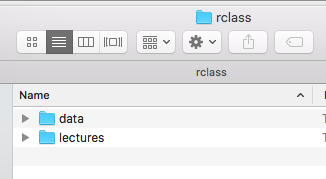
\includegraphics{rclass_folder.png}
\caption{}
\end{figure}

\end{frame}

\begin{frame}{Rclass folder structure}

\begin{itemize}
\tightlist
\item
  Inside the data subfolder, you should have the following subfolders:\\
  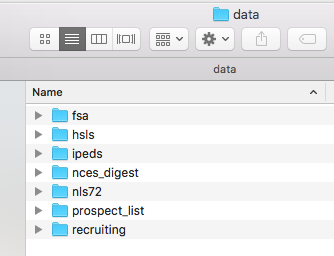
\includegraphics{rclass_folder_contents.png}
\end{itemize}

\end{frame}

\begin{frame}[fragile]{Save data for lecture}

We will not be providing links to data in this lecture. Please save data
to the corresponding folders.

\begin{itemize}
\tightlist
\item
  First make sure to save \textbf{lecture8.Rmd} in your lectures folder

  \begin{itemize}
  \tightlist
  \item
    If you do not have class folder structure, you can download it
    \href{https://github.com/ozanj/rclass/raw/master/rclass_directory.zip}{here}
  \end{itemize}
\item
  Download and unzip data folder we are using for this lecture
  \href{https://github.com/ozanj/rclass/raw/master/lectures/lecture8/lecture8_data.zip}{here}
\item
  Save data files in the corresponding data folder

  \begin{itemize}
  \tightlist
  \item
    \texttt{ipeds\_hd\_2017\_small.csv} should go in the \textbf{ic}
    folder inside the ipeds folder\\
  \item
    \texttt{peps300.xlsx} should go in the \textbf{fsa} folder\\
  \item
    \texttt{hsls\_sch\_small.dta} should go in the \textbf{hsls} folder
  \end{itemize}
\end{itemize}

\end{frame}

\begin{frame}[fragile]{Working directory}

\begin{itemize}
\tightlist
\item
  Your working directory will change depending on if you are using an R
  script or R markdown.
\item
  \textbf{R script}

  \begin{itemize}
  \tightlist
  \item
    The default working directory is your computer's home directory
  \item
    You only need to set your working directory \texttt{setwd()} in an r
    script once.\\
  \end{itemize}
\item
  \textbf{R markdown}

  \begin{itemize}
  \tightlist
  \item
    The default working directory is where the current r markdown file
    you are using is saved.\\
  \item
    If you set your working directory in a code chunk, it will be reset
    to the default directory after the code chunk is finished running.\\
  \item
    To avoid setting your working directory every time you read in data,
    you can read in data using a link to the data file or use the
    relative file path to save time.\\
  \end{itemize}
\item
  \textbf{R project}

  \begin{itemize}
  \tightlist
  \item
    The default working directory is in the R project location\\
  \item
    If you are working with an R script in an R project, the working
    directory is the R project main folder (ex. rclass)\\
  \item
    If you are working with an R markdown file in an R project, the
    working directory will be wherever the R markdown file is saved
    inside the R project.

    \begin{itemize}
    \tightlist
    \item
      For example, you have an R markdown file saved inside the lectures
      folder in an R project ``rclass'', your working directory may look
      like this (``/Users/pm/Desktop/rclass/lectures'')
    \end{itemize}
  \end{itemize}
\end{itemize}

\end{frame}

\begin{frame}[fragile]{Absolute vs.~relative filepath}

\textbf{Absolute file path}: The absolute file path is the complete list
of directories needed to locate a file or folder.\\
\texttt{setwd("/Users/pm/Desktop/rclass/lectures/lecture8")}

\textbf{Relative file path}: The relative file path is the path relative
to your current location/directory. Assuming your current working
directory is in the ``lecture8'' folder and you want to change your
directory to the data folder, your relative file path would look
something like this:\\
\texttt{setwd("../../data")}

\textbf{File path shortcuts}

\begin{longtable}[]{@{}ll@{}}
\toprule
\textbf{Key} & \textbf{Description}\tabularnewline
\midrule
\endhead
\textasciitilde{} & tilde is a shortcut for mac user's home directory
(mine is my name pm)\tabularnewline
../ & moves up a level\tabularnewline
../../ & moves up two level\tabularnewline
\bottomrule
\end{longtable}

\end{frame}

\begin{frame}[fragile]{Practice using relative file paths}

\begin{enumerate}
\def\labelenumi{\arabic{enumi}.}
\item
  Using the code chunk below, get your working directory
  \texttt{getwd()}
\item
  Using your relative file path, set your working directory to fsa
  folder inside the data folder. \texttt{setwd("filepath")}
\item
  Using your relative file path, set your working directory to the ef
  folder inside the ipeds folder inside the data folder.
  \texttt{setwd("filepath")}
\end{enumerate}

\end{frame}

\section{Common data formats}\label{common-data-formats}

\begin{frame}{Common data formats}

\begin{longtable}[]{@{}llll@{}}
\toprule
\textbf{Format} & \textbf{Package} & \textbf{Function} &\tabularnewline
\midrule
\endhead
Comma-separated values (.csv) & readr & read\_csv &\tabularnewline
Text-formated data (.txt) & readr & read\_table &\tabularnewline
Tab-separated values (.tsv) & readr & read\_tsv &\tabularnewline
Stata (.dta) & haven & read\_dta &\tabularnewline
SPSS (.sav) & haven & read\_sav &\tabularnewline
SAS (.sas) & haven & read\_sas &\tabularnewline
Excel (.xls or .xlsx) & readxl & read\_excel &\tabularnewline
R (.Rdata or .rds) & base R & load() &\tabularnewline
\bottomrule
\end{longtable}

\begin{itemize}
\tightlist
\item
  Source: Professor Darin Christensen
\end{itemize}

\end{frame}

\section{readr package}\label{readr-package}

\begin{frame}{readr}

The readr package is part of
\href{https://readr.tidyverse.org/index.html}{tidyverse}, which is
designed to read in flat data files in R and transform them into data
frames.\\[2\baselineskip]- We could load \textbf{library(tidyverse)} if
we wanted to load all packages in tidyverse (e.g.~ggplot2, dplyr, tidyr,
stringr, readr, etc\ldots{})

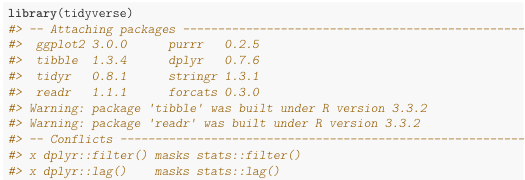
\includegraphics{tidyverse.png}\\
- For the purpose of this lecture, we will just need to load
\textbf{library(readr)}

\end{frame}

\subsection{readr functions}\label{readr-functions}

\begin{frame}[fragile]{readr functions}

\texttt{readr} (tidyverse) functions

Refer to the \texttt{readr} package
\href{https://cran.r-project.org/web/packages/readr/readr.pdf}{pdf} for
more detailed information on each function.\\
- Note: All of these functions follow similar syntax/rules in
\texttt{readr}

\begin{longtable}[]{@{}ll@{}}
\toprule
\textbf{Format} & \textbf{Function}\tabularnewline
\midrule
\endhead
Comma-separated values (csv) & \texttt{read\_csv}\tabularnewline
Semicolon separated files & \texttt{read\_csv2}\tabularnewline
Tab-separated values (tsv) & \texttt{read\_tsv}\tabularnewline
Any delimiter & \texttt{read\_delim}\tabularnewline
Fixed width files & \texttt{read\_fwf}\tabularnewline
Text-formated data (txt) & \texttt{read\_table}\tabularnewline
Web log files & \texttt{read\_log}\tabularnewline
\bottomrule
\end{longtable}

\end{frame}

\subsection{readr arguments}\label{readr-arguments}

\begin{frame}[fragile]{readr arguments}

\textbf{Arguments}

\begin{itemize}
\tightlist
\item
  \texttt{col\_types}: One of NULL, a cols() specification, or a string:

  \begin{itemize}
  \tightlist
  \item
    If NULL, all column types will be imputed from the first 1000 rows
    on the input. This is convenient (and fast), but not robust. If the
    imputation fails, you'll need to supply the correct types
    yourself.\\
  \item
    If a column specification created by cols(), it must contain one
    column specification for each column. If you only want to read a
    subset of the columns, use cols\_only().
  \end{itemize}
\item
  \texttt{skip}: Number of lines to skip before reading data.
\item
  \texttt{comment}: A string used to identify comments.
\item
  \texttt{col\_names}: Either TRUE, FALSE or a character vector of
  column names.

  \begin{itemize}
  \tightlist
  \item
    If TRUE, the first row of the input will be used as the column
    names, and will not be included in the data frame.\\
  \item
    If FALSE, column names will be generated automatically: X1, X2, X3
    etc.\\
  \item
    If col\_names is a character vector, the values will be used as the
    names of the columns, and the first row of the input will be read
    into the first row of the output data frame.
  \end{itemize}
\item
  \texttt{na}: Character vector of strings to use for missing values
\end{itemize}

\end{frame}

\subsection{readr column
specification}\label{readr-column-specification}

\begin{frame}[fragile]{readr column specification, part 1}

\texttt{readr} is pretty good at guessing each column's data type by
looking at the first 1,000 rows (e.g.~character, double, etc.), however
it is good practice to manually specify the data type for each column.

\begin{Shaded}
\begin{Highlighting}[]
\NormalTok{mtcars <-}\StringTok{ }\KeywordTok{read_csv}\NormalTok{(}\KeywordTok{readr_example}\NormalTok{(}\StringTok{"mtcars.csv"}\NormalTok{))}
\CommentTok{#> Parsed with column specification:}
\CommentTok{#> cols(}
\CommentTok{#>   mpg = col_double(),}
\CommentTok{#>   cyl = col_integer(),}
\CommentTok{#>   disp = col_double(),}
\CommentTok{#>   hp = col_integer(),}
\CommentTok{#>   drat = col_double(),}
\CommentTok{#>   wt = col_double(),}
\CommentTok{#>   qsec = col_double(),}
\CommentTok{#>   vs = col_integer(),}
\CommentTok{#>   am = col_integer(),}
\CommentTok{#>   gear = col_integer(),}
\CommentTok{#>   carb = col_integer()}
\CommentTok{#> )}
\end{Highlighting}
\end{Shaded}

\end{frame}

\begin{frame}[fragile]{readr column specification, part 1}

The output of the previous example shows us the column specification
readr gave us. However, we could manually change column specification if
we do not like readr's guess.

\begin{Shaded}
\begin{Highlighting}[]
\NormalTok{mtcars <-}\StringTok{ }\KeywordTok{read_csv}\NormalTok{(}\KeywordTok{readr_example}\NormalTok{(}\StringTok{"mtcars.csv"}\NormalTok{), }\DataTypeTok{col_types =} 
  \KeywordTok{cols}\NormalTok{(}
    \DataTypeTok{mpg =} \KeywordTok{col_double}\NormalTok{(),}
    \DataTypeTok{cyl =} \KeywordTok{col_integer}\NormalTok{(),}
    \DataTypeTok{disp =} \KeywordTok{col_double}\NormalTok{(),}
    \DataTypeTok{hp =} \KeywordTok{col_integer}\NormalTok{(),}
    \DataTypeTok{drat =} \KeywordTok{col_double}\NormalTok{(),}
    \DataTypeTok{vs =} \KeywordTok{col_integer}\NormalTok{(),}
    \DataTypeTok{wt =} \KeywordTok{col_double}\NormalTok{(),}
    \DataTypeTok{qsec =} \KeywordTok{col_double}\NormalTok{(),}
    \DataTypeTok{am =} \KeywordTok{col_integer}\NormalTok{(),}
    \DataTypeTok{gear =} \KeywordTok{col_integer}\NormalTok{(),}
    \DataTypeTok{carb =} \KeywordTok{col_integer}\NormalTok{()}
\NormalTok{  )}
\NormalTok{)}
\end{Highlighting}
\end{Shaded}

\end{frame}

\begin{frame}[fragile]{readr column specification, part 2}

\begin{longtable}[]{@{}ll@{}}
\toprule
\textbf{Data type} & \textbf{Arguments}\tabularnewline
\midrule
\endhead
Logical (TRUE \& FALSE) & \texttt{col\_logical()}\tabularnewline
Integers & \texttt{col\_integer()}\tabularnewline
Doubles & \texttt{col\_double()}\tabularnewline
Dates & \texttt{col\_date()}\tabularnewline
Characters & \texttt{col\_character()}\tabularnewline
Numbers & \texttt{col\_numeric()}\tabularnewline
Factors & \texttt{col\_factors(levels,\ ordered)}\tabularnewline
\bottomrule
\end{longtable}

\begin{Shaded}
\begin{Highlighting}[]
\KeywordTok{read_csv}\NormalTok{(}\StringTok{"a, b, c}
\StringTok{         1,2,F}
\StringTok{         4,5,T"}\NormalTok{, }\DataTypeTok{col_types =}
           \KeywordTok{cols}\NormalTok{(}
             \DataTypeTok{a =} \KeywordTok{col_factor}\NormalTok{(}\KeywordTok{c}\NormalTok{(}\StringTok{"1"}\NormalTok{, }\StringTok{"2"}\NormalTok{, }\StringTok{"3"}\NormalTok{, }\StringTok{"4"}\NormalTok{)),}
             \DataTypeTok{b =} \KeywordTok{col_character}\NormalTok{(),}
             \DataTypeTok{c =} \KeywordTok{col_logical}\NormalTok{()}
\NormalTok{           ))}
\CommentTok{#> # A tibble: 2 x 3}
\CommentTok{#>   a     b     c    }
\CommentTok{#>   <fct> <chr> <lgl>}
\CommentTok{#> 1 1     2     FALSE}
\CommentTok{#> 2 4     5     TRUE}
\end{Highlighting}
\end{Shaded}

\end{frame}

\begin{frame}[fragile]{readr demonstration csv}

\texttt{readr} automatically treats the first line of data as column
names.

\begin{Shaded}
\begin{Highlighting}[]
\KeywordTok{read_csv}\NormalTok{(}\StringTok{"column 1, column 2, column 3}
\StringTok{         1,2,3}
\StringTok{         4,5,6"}\NormalTok{, }\DataTypeTok{na =} \KeywordTok{c}\NormalTok{(}\DecValTok{2}\NormalTok{, }\StringTok{"NA"}\NormalTok{)}
\NormalTok{         )}
\CommentTok{#> # A tibble: 2 x 3}
\CommentTok{#>   `column 1` `column 2` `column 3`}
\CommentTok{#>        <int>      <int>      <int>}
\CommentTok{#> 1          1         NA          3}
\CommentTok{#> 2          4          5          6}
\end{Highlighting}
\end{Shaded}

There are instances where you may want to tell R from what line to begin
reading in data.

\end{frame}

\begin{frame}[fragile]{readr skip argument}

Notice the example below. The first two lines are comments about the
data. We would need to use \textbf{skip = n} to skip n lines.

\begin{Shaded}
\begin{Highlighting}[]
\KeywordTok{read_csv}\NormalTok{(}\StringTok{"This file contains data on student charges for the acdemic year.}
\StringTok{         File name: IC2016_AY}
\StringTok{         a, b, c}
\StringTok{         1,2,3}
\StringTok{         4,5,6"}\NormalTok{, }\DataTypeTok{skip =} \DecValTok{2}
\NormalTok{         )}
\CommentTok{#> # A tibble: 2 x 3}
\CommentTok{#>       a     b     c}
\CommentTok{#>   <int> <int> <int>}
\CommentTok{#> 1     1     2     3}
\CommentTok{#> 2     4     5     6}
\end{Highlighting}
\end{Shaded}

\end{frame}

\begin{frame}[fragile]{readr comment argument}

We could also tell R to drop lines we specify as comments. With
\textbf{comment = n}

\begin{Shaded}
\begin{Highlighting}[]
\KeywordTok{read_csv}\NormalTok{(}\StringTok{"# This file contains data on student charges for the acdemic year.}
\StringTok{         a, b, c}
\StringTok{         1,2,3}
\StringTok{         4,5,6"}\NormalTok{, }\DataTypeTok{comment =} \StringTok{"#"}
\NormalTok{         )}
\CommentTok{#> # A tibble: 2 x 3}
\CommentTok{#>       a     b     c}
\CommentTok{#>   <int> <int> <int>}
\CommentTok{#> 1     1     2     3}
\CommentTok{#> 2     4     5     6}
\end{Highlighting}
\end{Shaded}

\begin{Shaded}
\begin{Highlighting}[]
\KeywordTok{read_csv}\NormalTok{(}\StringTok{"* This file contains data on student charges for the acdemic year.}
\StringTok{         a, b, c}
\StringTok{         1,2,3}
\StringTok{         4,5,6"}\NormalTok{, }\DataTypeTok{comment =} \StringTok{"*"}
\NormalTok{         )}
\CommentTok{#> # A tibble: 2 x 3}
\CommentTok{#>       a     b     c}
\CommentTok{#>   <int> <int> <int>}
\CommentTok{#> 1     1     2     3}
\CommentTok{#> 2     4     5     6}
\end{Highlighting}
\end{Shaded}

\end{frame}

\begin{frame}[fragile]{readr column names argument}

We could tell R there are no column names with \textbf{col\_names =
FALSE} or we could manually give R column names with \textbf{col\_names
= c(``'', ``'', ``'')}

\begin{Shaded}
\begin{Highlighting}[]
\KeywordTok{read_csv}\NormalTok{(}\StringTok{"1,2,3}
\StringTok{         4,5,6"}\NormalTok{, }\DataTypeTok{col_names =} \OtherTok{FALSE}
\NormalTok{         )}
\CommentTok{#> # A tibble: 2 x 3}
\CommentTok{#>      X1    X2    X3}
\CommentTok{#>   <int> <int> <int>}
\CommentTok{#> 1     1     2     3}
\CommentTok{#> 2     4     5     6}
\end{Highlighting}
\end{Shaded}

\begin{Shaded}
\begin{Highlighting}[]
\KeywordTok{read_csv}\NormalTok{(}\StringTok{"1,2,3}
\StringTok{         4,5,6"}\NormalTok{, }\DataTypeTok{col_names =} \KeywordTok{c}\NormalTok{(}\StringTok{"column 1"}\NormalTok{, }\StringTok{"column 2"}\NormalTok{, }\StringTok{"column 3"}\NormalTok{)}
\NormalTok{         )}
\CommentTok{#> # A tibble: 2 x 3}
\CommentTok{#>   `column 1` `column 2` `column 3`}
\CommentTok{#>        <int>      <int>      <int>}
\CommentTok{#> 1          1          2          3}
\CommentTok{#> 2          4          5          6}
\end{Highlighting}
\end{Shaded}

\begin{Shaded}
\begin{Highlighting}[]
\KeywordTok{read_csv}\NormalTok{(}\StringTok{"a,b,c}
\StringTok{          1,2,3}
\StringTok{         4,5,6"}\NormalTok{, }\DataTypeTok{col_names =} \KeywordTok{c}\NormalTok{(}\StringTok{"column 1"}\NormalTok{, }\StringTok{"column 2"}\NormalTok{, }\StringTok{"column 3"}\NormalTok{), }\DataTypeTok{skip =} \DecValTok{1}
\NormalTok{         )}
\CommentTok{#> # A tibble: 2 x 3}
\CommentTok{#>   `column 1` `column 2` `column 3`}
\CommentTok{#>        <int>      <int>      <int>}
\CommentTok{#> 1          1          2          3}
\CommentTok{#> 2          4          5          6}
\end{Highlighting}
\end{Shaded}

\end{frame}

\begin{frame}[fragile]{readr Student exercise}

\begin{enumerate}
\def\labelenumi{\arabic{enumi}.}
\item
  Create a 3x3 tibble like the examples above
  (e.g.~read\_csv(``a,b,c\ldots{}.'')), treating the first line as
  column names
\item
  Now on the first line add a sentence and use the \texttt{skip}
  argument to skip this line
\item
  This time add a special character ( *, \#, ! ) at the beginning of the
  sentence and indicate it is a comment
\item
  Delete the sentence and column names (should have a 2x2 tibble) and
  manually tell R column names
\end{enumerate}

\end{frame}

\begin{frame}[fragile]{readr Student exercise solutions}

\begin{enumerate}
\def\labelenumi{\arabic{enumi}.}
\tightlist
\item
  Create a 3x3 tibble like the examples above
  (e.g.~read\_csv(``a,b,c\ldots{}.'')), treating the first line as
  column names
\end{enumerate}

\begin{Shaded}
\begin{Highlighting}[]
\KeywordTok{read_csv}\NormalTok{(}\StringTok{"a, b, c}
\StringTok{         1,2,3}
\StringTok{         4,5,6"}
\NormalTok{         )}
\CommentTok{#> # A tibble: 2 x 3}
\CommentTok{#>       a     b     c}
\CommentTok{#>   <int> <int> <int>}
\CommentTok{#> 1     1     2     3}
\CommentTok{#> 2     4     5     6}
\end{Highlighting}
\end{Shaded}

\begin{enumerate}
\def\labelenumi{\arabic{enumi}.}
\setcounter{enumi}{1}
\tightlist
\item
  Now on the first line add a sentence and use the \texttt{skip}
  argument to skip this line
\end{enumerate}

\begin{Shaded}
\begin{Highlighting}[]
\KeywordTok{read_csv}\NormalTok{(}\StringTok{"Do not read this sentence}
\StringTok{         a, b, c}
\StringTok{         1,2,3}
\StringTok{         4,5,6"}\NormalTok{, }\DataTypeTok{skip =} \DecValTok{1}
\NormalTok{         )}
\CommentTok{#> # A tibble: 2 x 3}
\CommentTok{#>       a     b     c}
\CommentTok{#>   <int> <int> <int>}
\CommentTok{#> 1     1     2     3}
\CommentTok{#> 2     4     5     6}
\end{Highlighting}
\end{Shaded}

\end{frame}

\begin{frame}[fragile]{readr Student exercise solutions continued}

\begin{enumerate}
\def\labelenumi{\arabic{enumi}.}
\setcounter{enumi}{2}
\tightlist
\item
  This time add a special character ( *, \#, ! ) at the beginning of the
  sentence and indicate it is a comment
\end{enumerate}

\begin{Shaded}
\begin{Highlighting}[]
\KeywordTok{read_csv}\NormalTok{(}\StringTok{"#This is a comment}
\StringTok{         a, b, c}
\StringTok{         1,2,3}
\StringTok{         4,5,6"}\NormalTok{,}\DataTypeTok{comment =} \StringTok{"#"}
\NormalTok{         )}
\CommentTok{#> # A tibble: 2 x 3}
\CommentTok{#>       a     b     c}
\CommentTok{#>   <int> <int> <int>}
\CommentTok{#> 1     1     2     3}
\CommentTok{#> 2     4     5     6}
\end{Highlighting}
\end{Shaded}

\begin{enumerate}
\def\labelenumi{\arabic{enumi}.}
\setcounter{enumi}{3}
\tightlist
\item
  Delete the sentence and column names (should have a 2x3 tibble) and
  manually tell R column names
\end{enumerate}

\begin{Shaded}
\begin{Highlighting}[]
\KeywordTok{read_csv}\NormalTok{(}\StringTok{"1,2,3}
\StringTok{         4,5,6"}\NormalTok{,}\DataTypeTok{col_names =} \KeywordTok{c}\NormalTok{(}\StringTok{"a"}\NormalTok{, }\StringTok{"b"}\NormalTok{, }\StringTok{"c"}\NormalTok{)}
\NormalTok{         )}
\CommentTok{#> # A tibble: 2 x 3}
\CommentTok{#>       a     b     c}
\CommentTok{#>   <int> <int> <int>}
\CommentTok{#> 1     1     2     3}
\CommentTok{#> 2     4     5     6}
\end{Highlighting}
\end{Shaded}

\end{frame}

\begin{frame}[fragile]{1. readr Running into errors}

\begin{enumerate}
\def\labelenumi{\arabic{enumi}.}
\tightlist
\item
  Make sure you have downloaded and saved the flat file\\
\item
  Make sure to know the file path of where data is downloaded or saved
  (``../../data'')

  \begin{itemize}
  \tightlist
  \item
    You can use the \texttt{list.files()} function to view what files
    you have in a particular folder
  \end{itemize}
\item
  Make sure you set your working \textbf{\texttt{setwd()}} directory in
  R. To check your current working directory type
  \textbf{\texttt{getwd()}} in console.
\end{enumerate}

\end{frame}

\begin{frame}{read\_csv demonstration using IPEDS data}

Integrated Postsecondary Education Data System (IPEDS)

\begin{itemize}
\tightlist
\item
  Postsecondary education data from NCES\\
\item
  There are
  \href{https://nces.ed.gov/ipeds/resource/download/IPEDS_DataReleaseProcedures.pdf}{12
  survey components} and 3 collection periods
\end{itemize}

We will be working with
\href{https://nces.ed.gov/ipeds/datacenter/DataFiles.aspx}{Institutional
Characteristics data of 2017}

\end{frame}

\begin{frame}[fragile]{read\_csv demonstration using IPEDS data}

\textbf{Tying it all together}

Use \texttt{read\_csv()} function from \texttt{readr} to import csv
dataset into R without column specification. Follow along on your
computers.

\begin{Shaded}
\begin{Highlighting}[]
\NormalTok{ipeds <-}\StringTok{ }\KeywordTok{read_csv}\NormalTok{(}\DataTypeTok{file=}\StringTok{"../../data/ipeds/ic/ipeds_hd_2017_small.csv"}\NormalTok{)}
\CommentTok{#> Parsed with column specification:}
\CommentTok{#> cols(}
\CommentTok{#>   unitid = col_integer(),}
\CommentTok{#>   instnm = col_character(),}
\CommentTok{#>   stabbr = col_character(),}
\CommentTok{#>   sector = col_integer(),}
\CommentTok{#>   iclevel = col_integer(),}
\CommentTok{#>   control = col_integer()}
\CommentTok{#> )}
\CommentTok{# glimpse(ipeds)}
\end{Highlighting}
\end{Shaded}

\end{frame}

\begin{frame}[fragile]{read\_csv demonstration using IPEDS data}

Use \texttt{read\_csv()} function from \texttt{readr} to import csv
dataset into R with column specification

\begin{Shaded}
\begin{Highlighting}[]

\NormalTok{ipeds <-}\StringTok{ }\KeywordTok{read_csv}\NormalTok{(}\DataTypeTok{file=}\StringTok{"../../data/ipeds/ic/ipeds_hd_2017_small.csv"}\NormalTok{,}
                  \DataTypeTok{col_types =}
                    \KeywordTok{cols}\NormalTok{(}
                      \DataTypeTok{unitid =} \KeywordTok{col_character}\NormalTok{(), }
                      \DataTypeTok{instnm =} \KeywordTok{col_character}\NormalTok{(),}
                      \DataTypeTok{stabbr =} \KeywordTok{col_character}\NormalTok{(),}
                      \DataTypeTok{sector =} \KeywordTok{col_integer}\NormalTok{(),}
                      \DataTypeTok{iclevel =} \KeywordTok{col_integer}\NormalTok{(),}
                      \DataTypeTok{control =} \KeywordTok{col_integer}\NormalTok{()}
\NormalTok{  )}
\NormalTok{)}
\end{Highlighting}
\end{Shaded}

We changed unitid to number, but could be left as is or changed to
character type for example.

\end{frame}

\begin{frame}[fragile]{readr variable and value labels}

Let's view variable and value labels

\begin{Shaded}
\begin{Highlighting}[]
\NormalTok{ipeds }\OperatorTok\StringTok{ }\KeywordTok{select}\NormalTok{(sector) }\OperatorTok\StringTok{ }\KeywordTok{var_label}\NormalTok{()}
\CommentTok{#> $sector}
\CommentTok{#> NULL}
\NormalTok{ipeds }\OperatorTok\StringTok{ }\KeywordTok{select}\NormalTok{(sector) }\OperatorTok\StringTok{ }\KeywordTok{val_labels}\NormalTok{()}
\CommentTok{#> $sector}
\CommentTok{#> NULL}
\end{Highlighting}
\end{Shaded}

\begin{itemize}
\item
  There are no variable and value labels for this data. IPEDS has a
  separate do file with variable and value labels.
\item
  Let's practice manually adding variable and value labels using the
  \texttt{labelled} package.
\end{itemize}

\end{frame}

\section{Set variable and value
labels}\label{set-variable-and-value-labels}

\begin{frame}[fragile]{Set variable and value labels}

Let's create a tibble first

\begin{Shaded}
\begin{Highlighting}[]
\NormalTok{df <-}\StringTok{ }\KeywordTok{tribble}\NormalTok{(}
  \OperatorTok{~}\NormalTok{id, }\OperatorTok{~}\NormalTok{edu, }\OperatorTok{~}\NormalTok{sch,}
  \CommentTok{#--|--|----}
  \DecValTok{1}\NormalTok{, }\DecValTok{2}\NormalTok{, }\DecValTok{2}\NormalTok{,}
  \DecValTok{2}\NormalTok{, }\DecValTok{1}\NormalTok{, }\DecValTok{1}\NormalTok{,}
  \DecValTok{3}\NormalTok{, }\DecValTok{3}\NormalTok{, }\DecValTok{2}\NormalTok{,}
  \DecValTok{4}\NormalTok{, }\DecValTok{4}\NormalTok{, }\DecValTok{2}\NormalTok{,}
  \DecValTok{5}\NormalTok{, }\DecValTok{1}\NormalTok{, }\DecValTok{2}
\NormalTok{)}
\NormalTok{df}
\CommentTok{#> # A tibble: 5 x 3}
\CommentTok{#>      id   edu   sch}
\CommentTok{#>   <dbl> <dbl> <dbl>}
\CommentTok{#> 1     1     2     2}
\CommentTok{#> 2     2     1     1}
\CommentTok{#> 3     3     3     2}
\CommentTok{#> 4     4     4     2}
\CommentTok{#> 5     5     1     2}
\end{Highlighting}
\end{Shaded}

\end{frame}

\begin{frame}[fragile]{Set variable labels}

\begin{itemize}
\tightlist
\item
  Use \texttt{set\_variable\_labels} function to manually set variable
  labels

  \begin{itemize}
  \tightlist
  \item
    \texttt{df\ \%\textgreater{}\%\ set\_variable\_labels(variable\ =\ "Variable\ label")}\\
  \item
    \texttt{ipeds\ \%\textgreater{}\%\ set\_variable\_labels(unitid\ =\ "Unit\ identification\ number")}
  \end{itemize}
\end{itemize}

\begin{Shaded}
\begin{Highlighting}[]
\KeywordTok{class}\NormalTok{(df}\OperatorTok{$}\NormalTok{sch)}
\CommentTok{#> [1] "numeric"}
\NormalTok{df <-}\StringTok{ }\NormalTok{df }\OperatorTok
\StringTok{  }\KeywordTok{set_variable_labels}\NormalTok{(}
    \DataTypeTok{id =} \StringTok{"Unique identification number"}\NormalTok{,}
    \DataTypeTok{edu =} \StringTok{"Education level"}\NormalTok{,}
    \DataTypeTok{sch =} \StringTok{"Type of school attending"}
\NormalTok{  )}
\KeywordTok{class}\NormalTok{(df}\OperatorTok{$}\NormalTok{sch)}
\CommentTok{#> [1] "numeric"}
\end{Highlighting}
\end{Shaded}

\end{frame}

\begin{frame}[fragile]{Set value labels}

\begin{itemize}
\tightlist
\item
  Use \texttt{set\_value\_labels} function to manually set value labels

  \begin{itemize}
  \tightlist
  \item
    \texttt{df\ \%\textgreater{}\%\ set\_value\_labels(variable\ =\ c("Value\ label"\ =\ 1,\ "Value\ label"\ =\ 2))}\\
  \item
    \texttt{ipeds\ \%\textgreater{}\%\ set\_value\_labels(sector\ =\ "Administrative\ Unit"\ =\ 0)}
  \end{itemize}
\end{itemize}

\begin{Shaded}
\begin{Highlighting}[]
\KeywordTok{class}\NormalTok{(df}\OperatorTok{$}\NormalTok{sch)}
\CommentTok{#> [1] "numeric"}
\NormalTok{df <-}\StringTok{ }\NormalTok{df }\OperatorTok
\StringTok{  }\KeywordTok{set_value_labels}\NormalTok{(}
    \DataTypeTok{edu =} \KeywordTok{c}\NormalTok{(}\StringTok{"High School"}\NormalTok{ =}\StringTok{ }\DecValTok{1}\NormalTok{,}
            \StringTok{"AA degree"}\NormalTok{ =}\StringTok{ }\DecValTok{2}\NormalTok{,}
            \StringTok{"BA degree"}\NormalTok{ =}\StringTok{ }\DecValTok{3}\NormalTok{,}
            \StringTok{"MA or higher"}\NormalTok{ =}\StringTok{ }\DecValTok{4}\NormalTok{),}
    \DataTypeTok{sch =} \KeywordTok{c}\NormalTok{(}\StringTok{"Private"}\NormalTok{ =}\StringTok{ }\DecValTok{1}\NormalTok{,}
            \StringTok{"Public"}\NormalTok{ =}\StringTok{ }\DecValTok{2}\NormalTok{))}
\KeywordTok{class}\NormalTok{(df}\OperatorTok{$}\NormalTok{sch)}
\CommentTok{#> [1] "labelled"}
\end{Highlighting}
\end{Shaded}

\end{frame}

\begin{frame}[fragile]{readr labelled data}

\begin{itemize}
\tightlist
\item
  Open the data dictionary file for
  \href{https://nces.ed.gov/ipeds/datacenter/data/HD2017_Dict.zip}{hd2017}
  data and select ``Frequencies'' sheet
\item
  We are only working with these 6 variables (unitid, instnm, stabbr,
  sector, iclevel, control)
\end{itemize}

\begin{Shaded}
\begin{Highlighting}[]
\CommentTok{# Lets view values for sector}
\NormalTok{ipeds }\OperatorTok
\StringTok{  }\KeywordTok{count}\NormalTok{(sector) }
\CommentTok{#> # A tibble: 11 x 2}
\CommentTok{#>    sector     n}
\CommentTok{#>     <int> <int>}
\CommentTok{#>  1      0    75}
\CommentTok{#>  2      1   775}
\CommentTok{#>  3      2  1701}
\CommentTok{#>  4      3   661}
\CommentTok{#>  5      4   981}
\CommentTok{#>  6      5   169}
\CommentTok{#>  7      6   864}
\CommentTok{#>  8      7   248}
\CommentTok{#>  9      8    85}
\CommentTok{#> 10      9  1562}
\CommentTok{#> 11     99    32}
\end{Highlighting}
\end{Shaded}

\end{frame}

\begin{frame}{readr variable and value labels student exercise}

\begin{enumerate}
\def\labelenumi{\arabic{enumi}.}
\item
  Using the codebook for hd2017 data, add variable labels for all 6
  variables (unitid, instnm, stabbr, sector, iclevel, control)
\item
  Add value labels for sector, iclevel, and control
\end{enumerate}

\end{frame}

\begin{frame}[fragile]{readr variable and value labels student exercise
solution}

\begin{Shaded}
\begin{Highlighting}[]
\CommentTok{# Need to manually assign variable and value labels using labelled package }
\NormalTok{ipeds_labelled <-}\StringTok{ }\NormalTok{ipeds }\OperatorTok
\StringTok{  }\KeywordTok{set_variable_labels}\NormalTok{(}\DataTypeTok{unitid =} \StringTok{"Unit identification number"}\NormalTok{, }
                      \DataTypeTok{instnm =} \StringTok{"Institution name"}\NormalTok{, }
                      \DataTypeTok{stabbr =} \StringTok{"State abbreviation"}\NormalTok{,}
                      \DataTypeTok{sector =} \StringTok{"Sector of institution"}\NormalTok{,}
                      \DataTypeTok{iclevel =} \StringTok{"Level of institution"}\NormalTok{,}
                      \DataTypeTok{control =} \StringTok{"Control of institution"}\NormalTok{) }\OperatorTok
\StringTok{  }\KeywordTok{set_value_labels}\NormalTok{(}\DataTypeTok{sector =} \KeywordTok{c}\NormalTok{(}\StringTok{"Administrative Unit"}\NormalTok{ =}\StringTok{ }\DecValTok{0}\NormalTok{, }
                              \StringTok{"Public, 4-year or above"}\NormalTok{ =}\StringTok{ }\DecValTok{1}\NormalTok{, }
                              \StringTok{"Private not-for-profit, 4-year or above"}\NormalTok{ =}\StringTok{ }\DecValTok{2}\NormalTok{,}
                              \StringTok{"Private for-profit, 4-year or above"}\NormalTok{ =}\StringTok{ }\DecValTok{3}\NormalTok{, }
                              \StringTok{"Public, 2-year"}\NormalTok{ =}\StringTok{ }\DecValTok{4}\NormalTok{, }
                              \StringTok{"Private not-for-profit, 2-year"}\NormalTok{ =}\StringTok{ }\DecValTok{5}\NormalTok{, }
                              \StringTok{"Private for-profit, 2-year"}\NormalTok{ =}\StringTok{ }\DecValTok{6}\NormalTok{,}
                              \StringTok{"Public, less-than 2-year"}\NormalTok{ =}\StringTok{ }\DecValTok{7}\NormalTok{, }
                              \StringTok{"Private not-for-profit, less-than 2-year"}\NormalTok{ =}\StringTok{ }\DecValTok{8}\NormalTok{,}
                              \StringTok{"Private for-profit, less-than 2-year"}\NormalTok{ =}\StringTok{ }\DecValTok{9}\NormalTok{, }
                              \StringTok{"Sector unknown (not active)"}\NormalTok{ =}\StringTok{ }\DecValTok{99}\NormalTok{), }
                   \DataTypeTok{iclevel =} \KeywordTok{c}\NormalTok{(}\StringTok{"Four or more years"}\NormalTok{ =}\StringTok{ }\DecValTok{1}\NormalTok{, }
                               \StringTok{"At least 2 but less than 4 years"}\NormalTok{ =}\StringTok{ }\DecValTok{2}\NormalTok{, }
                               \StringTok{"Less than 2 years (below associate)"}\NormalTok{ =}\StringTok{ }\DecValTok{3}\NormalTok{,}
                               \StringTok{"\{Not available\}"}\NormalTok{ =}\StringTok{ }\OperatorTok{-}\DecValTok{3}\NormalTok{),}
                   \DataTypeTok{control =} \KeywordTok{c}\NormalTok{(}\StringTok{"Public"}\NormalTok{ =}\StringTok{ }\DecValTok{1}\NormalTok{, }\StringTok{"Private not-for-profit"}\NormalTok{ =}\StringTok{ }\DecValTok{2}\NormalTok{, }
                               \StringTok{"Private for-profit"}\NormalTok{ =}\StringTok{ }\DecValTok{3}\NormalTok{, }
                               \StringTok{"\{Not available\}"}\NormalTok{ =}\StringTok{ }\OperatorTok{-}\DecValTok{3}\NormalTok{))}
\end{Highlighting}
\end{Shaded}

\end{frame}

\begin{frame}[fragile]{readr Let's view new labelled data}

\begin{Shaded}
\begin{Highlighting}[]
\KeywordTok{typeof}\NormalTok{(ipeds_labelled}\OperatorTok{$}\NormalTok{iclevel)}
\CommentTok{#> [1] "integer"}
\KeywordTok{class}\NormalTok{(ipeds_labelled}\OperatorTok{$}\NormalTok{iclevel)}
\CommentTok{#> [1] "labelled"}
\KeywordTok{attributes}\NormalTok{(ipeds_labelled}\OperatorTok{$}\NormalTok{iclevel)}
\CommentTok{#> $label}
\CommentTok{#> [1] "Level of institution"}
\CommentTok{#> }
\CommentTok{#> $labels}
\CommentTok{#>                  Four or more years    At least 2 but less than 4 years }
\CommentTok{#>                                   1                                   2 }
\CommentTok{#> Less than 2 years (below associate)                     \{Not available\} }
\CommentTok{#>                                   3                                  -3 }
\CommentTok{#> }
\CommentTok{#> $class}
\CommentTok{#> [1] "labelled"}
\end{Highlighting}
\end{Shaded}

\end{frame}

\begin{frame}[fragile]{\texttt{as\_factor()} function}

\textbf{Usage (i.e., syntax)}:
\texttt{as\_factor(x,\ ...,\ only\_labelled\ =\ TRUE)}

\textbf{Arguments}

\begin{itemize}
\tightlist
\item
  \texttt{x}: object to coerce to a factor\\
\item
  \texttt{...}: other arguments passed down to method\\
\item
  \texttt{only\_labelled}: only apply to labelled columns\\
\item
  \texttt{levels}: How to create the levels of the generated factor:

  \begin{itemize}
  \tightlist
  \item
    ``default'': uses labels where available, otherwise the values.
    Labels are sorted by value.\\
  \item
    ``both'': like ``default'', but pastes together the level and
    value\\
  \item
    ``label'': use only the labels; unlabelled values become NA labelled
    3\\
  \item
    ``values: use only the values\\
  \end{itemize}
\item
  \texttt{ordered}: If TRUE create an ordered (ordinal) factor, if FALSE
  (the default) create a regular (nominal) factor
\end{itemize}

\textbf{Example}: Change labelled columns to factor

\begin{Shaded}
\begin{Highlighting}[]
\KeywordTok{as_factor}\NormalTok{(df, }\DataTypeTok{only_labelled =} \OtherTok{TRUE}\NormalTok{) }
\end{Highlighting}
\end{Shaded}

\end{frame}

\begin{frame}[fragile]{readr labelled data to factor}

Let's change class to factor

\begin{Shaded}
\begin{Highlighting}[]
\NormalTok{ipeds_factor <-}\StringTok{ }\KeywordTok{as_factor}\NormalTok{(ipeds_labelled, }\DataTypeTok{only_labelled =} \OtherTok{TRUE}\NormalTok{)}
\KeywordTok{typeof}\NormalTok{(ipeds_factor}\OperatorTok{$}\NormalTok{sector)}
\CommentTok{#> [1] "integer"}
\KeywordTok{class}\NormalTok{(ipeds_factor}\OperatorTok{$}\NormalTok{sector)}
\CommentTok{#> [1] "factor"}
\KeywordTok{attributes}\NormalTok{(ipeds_factor}\OperatorTok{$}\NormalTok{sector)}
\CommentTok{#> $levels}
\CommentTok{#>  [1] "Administrative Unit"                     }
\CommentTok{#>  [2] "Public, 4-year or above"                 }
\CommentTok{#>  [3] "Private not-for-profit, 4-year or above" }
\CommentTok{#>  [4] "Private for-profit, 4-year or above"     }
\CommentTok{#>  [5] "Public, 2-year"                          }
\CommentTok{#>  [6] "Private not-for-profit, 2-year"          }
\CommentTok{#>  [7] "Private for-profit, 2-year"              }
\CommentTok{#>  [8] "Public, less-than 2-year"                }
\CommentTok{#>  [9] "Private not-for-profit, less-than 2-year"}
\CommentTok{#> [10] "Private for-profit, less-than 2-year"    }
\CommentTok{#> [11] "Sector unknown (not active)"             }
\CommentTok{#> }
\CommentTok{#> $class}
\CommentTok{#> [1] "factor"}
\CommentTok{#> }
\CommentTok{#> $label}
\CommentTok{#> [1] "Sector of institution"}
\end{Highlighting}
\end{Shaded}

\end{frame}

\section{Reading in data from the
web}\label{reading-in-data-from-the-web}

\begin{frame}{Reading in data from the web}

\begin{itemize}
\tightlist
\item
  Save time

  \begin{itemize}
  \tightlist
  \item
    Reduce the steps of downloading, saving, and reading in data\\
  \item
    Read in data directly from internet\\
  \item
    \textbf{note} not all packages will working with downloading data
    from the web (read\_excel)
  \end{itemize}
\end{itemize}

For example, rather than downloading Raj Chetty data and saving it in a
folder, we could download the data directly from the web.

\end{frame}

\begin{frame}{Reading in data from web example using Raj Chetty data}

Equality of Opportunity Project

\begin{itemize}
\tightlist
\item
  \href{http://www.equality-of-opportunity.org/papers/coll_mrc_paper.pdf}{Equality
  of Opportunity Project} uses two data sources-- federal tax recoards
  and Department of Education records (1999-2013)-- to investigate
  intergenerational income mobility at colleges in the US.
\end{itemize}

We will use
\href{http://www.equality-of-opportunity.org/documents/}{Mobility Report
Cards: The Role of Colleges in Intergenerational Mobility data}

\end{frame}

\begin{frame}{Reading in data from web example using Raj Chetty data}

\begin{enumerate}
\def\labelenumi{\arabic{enumi}.}
\tightlist
\item
  Follow this \href{http://www.equality-of-opportunity.org/data/}{link}
  and under the ``Mobility Report Cards\ldots{}'' tab select ``click to
  view data''.\\
\item
  Choose ``Online Data Table 1''
\item
  Right click and copy link address for ``Excel'' (Note: it is actually
  a csv file)
\end{enumerate}

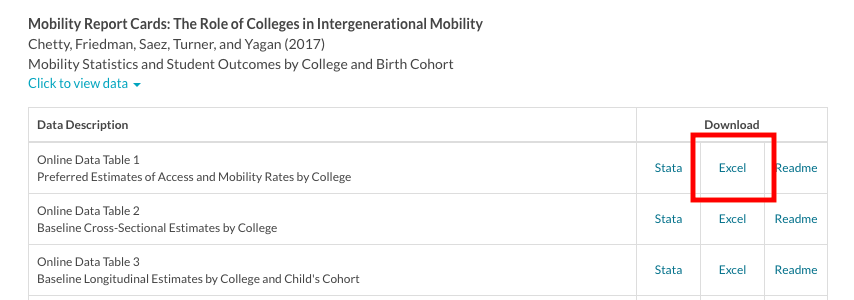
\includegraphics{mrc_table1.png}~

\end{frame}

\begin{frame}[fragile]{Reading in data from the web}

Approach \#1

\begin{Shaded}
\begin{Highlighting}[]
\CommentTok{#Paste url to excel "csv" file}
\NormalTok{data_url <-}\StringTok{ "http://www.equality-of-opportunity.org/data/college/mrc_table1.csv"}

\CommentTok{#Download data and read in using read_csv (readr)}
\NormalTok{mrc <-}\StringTok{ }\KeywordTok{read_csv}\NormalTok{(data_url)}

\CommentTok{#View first 4 rows and 4 columns }
\NormalTok{mrc[}\DecValTok{1}\OperatorTok{:}\DecValTok{4}\NormalTok{, }\DecValTok{1}\OperatorTok{:}\DecValTok{4}\NormalTok{]}
\CommentTok{#> # A tibble: 4 x 4}
\CommentTok{#>   super_opeid name                                         czname   state}
\CommentTok{#>         <int> <chr>                                        <chr>    <chr>}
\CommentTok{#> 1        2665 Vaughn College Of Aeronautics And Technology New York NY   }
\CommentTok{#> 2        7273 CUNY Bernard M. Baruch College               New York NY   }
\CommentTok{#> 3        2688 City College Of New York - CUNY              New York NY   }
\CommentTok{#> 4        7022 CUNY Lehman College                          New York NY}
\end{Highlighting}
\end{Shaded}

\end{frame}

\begin{frame}[fragile]{Reading in data from the web}

Approach \#2

\begin{Shaded}
\begin{Highlighting}[]
\CommentTok{#Download data and read in link directly using read_csv (readr)}
\NormalTok{mrc <-}\StringTok{ }\KeywordTok{read_csv}\NormalTok{(}\StringTok{"http://www.equality-of-opportunity.org/data/college/mrc_table1.csv"}\NormalTok{)}
\CommentTok{#> Parsed with column specification:}
\CommentTok{#> cols(}
\CommentTok{#>   super_opeid = col_integer(),}
\CommentTok{#>   name = col_character(),}
\CommentTok{#>   czname = col_character(),}
\CommentTok{#>   state = col_character(),}
\CommentTok{#>   par_median = col_integer(),}
\CommentTok{#>   k_median = col_integer(),}
\CommentTok{#>   par_q1 = col_double(),}
\CommentTok{#>   par_top1pc = col_double(),}
\CommentTok{#>   kq5_cond_parq1 = col_double(),}
\CommentTok{#>   ktop1pc_cond_parq1 = col_double(),}
\CommentTok{#>   mr_kq5_pq1 = col_double(),}
\CommentTok{#>   mr_ktop1_pq1 = col_double(),}
\CommentTok{#>   trend_parq1 = col_double(),}
\CommentTok{#>   trend_bottom40 = col_double(),}
\CommentTok{#>   count = col_double()}
\CommentTok{#> )}
\end{Highlighting}
\end{Shaded}

\end{frame}

\begin{frame}[fragile]{Reading in data from the web}

\begin{Shaded}
\begin{Highlighting}[]
\CommentTok{#View first 4 rows and 4 columns }
\NormalTok{mrc[}\DecValTok{1}\OperatorTok{:}\DecValTok{4}\NormalTok{, }\DecValTok{1}\OperatorTok{:}\DecValTok{4}\NormalTok{]}
\CommentTok{#> # A tibble: 4 x 4}
\CommentTok{#>   super_opeid name                                         czname   state}
\CommentTok{#>         <int> <chr>                                        <chr>    <chr>}
\CommentTok{#> 1        2665 Vaughn College Of Aeronautics And Technology New York NY   }
\CommentTok{#> 2        7273 CUNY Bernard M. Baruch College               New York NY   }
\CommentTok{#> 3        2688 City College Of New York - CUNY              New York NY   }
\CommentTok{#> 4        7022 CUNY Lehman College                          New York NY}
\end{Highlighting}
\end{Shaded}

\end{frame}

\begin{frame}{Problems downloading data (zip files) using IPEDS}

\begin{enumerate}
\def\labelenumi{\arabic{enumi}.}
\tightlist
\item
  Follow this \href{https://nces.ed.gov/ipeds/use-the-data}{link} and
  under the ``Survey Data'' tab select ``Complete data files''.\\
\item
  Choose ``All years'' and ``All surveys'' and click continue\\
\item
  Right click and copy link address for ``IC2017\_AY''
\end{enumerate}

\begin{figure}
\centering
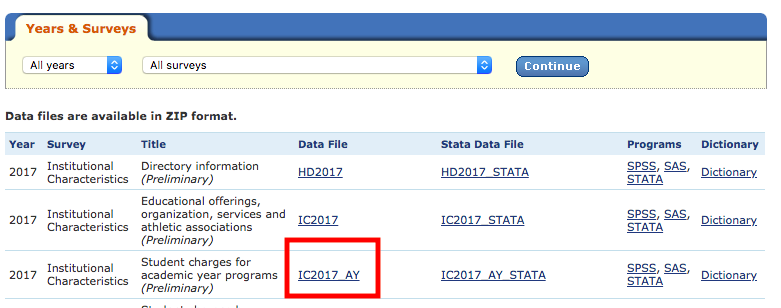
\includegraphics{ic2017_ay.png}
\caption{ipeds data center}
\end{figure}

\end{frame}

\begin{frame}[fragile]{Downloading data (zip files) using IPEDS}

\begin{itemize}
\tightlist
\item
  Paste url and read in using \texttt{read\_csv}

  \begin{itemize}
  \tightlist
  \item
    \texttt{ipeds\ \textless{}-\ read\_csv("link")} What happens when
    you try reading in this file?
  \end{itemize}
\end{itemize}

Need to download \textbf{and} unzip

\end{frame}

\subsection{download.file function}\label{download.file-function}

\begin{frame}[fragile]{download.file function}

\texttt{download.file} is a function use to download a file from the
internet.

\textbf{Usage (i.e., syntax)}:
\texttt{download.file(url,\ destfile,\ method,\ quiet\ =\ FALSE,\ mode\ =\ "w")}

\textbf{Arguments}

\begin{itemize}
\tightlist
\item
  \texttt{url}: A character string naming the URL of a resource to be
  downloaded\\
\item
  \texttt{destfile}: A character string with the name where the
  downloaded file is saved.\\
\item
  \texttt{method}: Method to be used for downloading files. Current
  download methods are ``internal'', ``wininet'' (Windows only)
  ``libcurl'', ``wget'' and ``curl'', and there is a value ``auto''\\
\item
  \texttt{quiet}: If TRUE, suppress status messages (if any), and the
  progress bar.\\
\item
  \texttt{mode}: character. The mode with which to write the file.
  Useful values are ``w'', ``wb'' (binary), ``a'' (append) and ``ab''.
  Not used for methods ``wget'' and ``curl''\\
\item
  \texttt{cacheOK}: logical. Is a server-side cached value acceptable?\\
\item
  \texttt{extra}: character vector of additional command-line arguments
  for the ``wget'' and ``curl'' methods.\\
\item
  \texttt{...}: allow additional arguments to be passed, unused
\end{itemize}

\end{frame}

\begin{frame}[fragile]{download.file function}

\textbf{Details}: The function download.file can be used to download a
single file as described by url from the internet and store it in
destfile. The url must start with a scheme such as \url{http://},
\url{https://}, \url{ftp://} or \url{file://}.

\textbf{Example}: Download data from the web

\begin{Shaded}
\begin{Highlighting}[]
\CommentTok{#Data from the Equality of Opportunity Project}
\KeywordTok{download.file}\NormalTok{(}\DataTypeTok{url =} \StringTok{"http://www.equality-of-opportunity.org/data/race/table_1.csv"}\NormalTok{,}
              \DataTypeTok{destfile =} \StringTok{"../../../../table_1.csv"}\NormalTok{, }\DataTypeTok{mode =} \StringTok{"wb"}\NormalTok{) }
\end{Highlighting}
\end{Shaded}

\end{frame}

\begin{frame}[fragile]{unzip files}

\texttt{unzip} is used to extract files from or list a zip archive.

\textbf{Usage (i.e., syntax)}:
\texttt{unzip(zipfile,\ files\ =\ NULL,\ list\ =\ FALSE,\ overwrite\ =\ TRUE,\ unzip\ =\ "internal",\ exdir\ =\ ".")}

\textbf{Arguments}

\begin{itemize}
\tightlist
\item
  \texttt{zipfile}: The pathname of the zip file
\item
  \texttt{files}: A character vector of recorded filepaths to be
  extracted: the default is to extract all files.\\
\item
  \texttt{list}: If TRUE, list the files and extract none.
\item
  \texttt{overwrite}: If TRUE, overwrite existing files, otherwise
  ignore such files.\\
\item
  \texttt{junkpaths}: If TRUE, use only the basename of the stored
  filepath when extracting.\\
\item
  \texttt{exdir}: The directory to extract files to
\item
  \texttt{unzip}: The method to be used.
\end{itemize}

\end{frame}

\begin{frame}[fragile]{Downloading data (zip files) using IPEDS}

\begin{Shaded}
\begin{Highlighting}[]
\CommentTok{#Set path to where data will be saved}
\CommentTok{#setwd()}
\CommentTok{#download file and pa}
\KeywordTok{download.file}\NormalTok{(}\StringTok{"https://nces.ed.gov/ipeds/datacenter/data/IC2017_AY.zip"}\NormalTok{,}
              \DataTypeTok{destfile =} \StringTok{"ic2017_ay"}\NormalTok{, }\DataTypeTok{mode =} \StringTok{"wb"}\NormalTok{)}
\CommentTok{#unzip zip file and keep original name}
\KeywordTok{unzip}\NormalTok{(}\DataTypeTok{zipfile =} \StringTok{"ic2017_ay"}\NormalTok{ , }\DataTypeTok{unzip =} \StringTok{"unzip"}\NormalTok{)}

\NormalTok{ic2017_ay <-}\StringTok{ }\KeywordTok{read_csv}\NormalTok{(}\StringTok{"ic2017_ay.csv"}\NormalTok{) }\OperatorTok
\StringTok{  }\KeywordTok{select}\NormalTok{(}\OperatorTok{-}\KeywordTok{starts_with}\NormalTok{(}\StringTok{"X"}\NormalTok{))}
\CommentTok{#> Parsed with column specification:}
\CommentTok{#> cols(}
\CommentTok{#>   .default = col_character(),}
\CommentTok{#>   UNITID = col_integer()}
\CommentTok{#> )}
\CommentTok{#> See spec(...) for full column specifications.}

\KeywordTok{names}\NormalTok{(ic2017_ay) <-}\StringTok{ }\KeywordTok{tolower}\NormalTok{(}\KeywordTok{names}\NormalTok{(ic2017_ay)) }\CommentTok{#lowercase column names}

\CommentTok{#names(ic2017_ay)}
\end{Highlighting}
\end{Shaded}

\end{frame}

\begin{frame}[fragile]{Student exercise}

\textbf{Tying it all together}

\begin{itemize}
\tightlist
\item
  Using everything we learned today, read in a csv data file from the
  web\\
\item
  Go back to the ipeds data center
  \href{https://nces.ed.gov/ipeds/datacenter/DataFiles.aspx}{here}\\
\item
  Right click and copy the link address to a different data file
  (``HD2017'', ``EFFY2017'')\\
\item
  Make sure to download the link first (download.file) before reading in
  the data\\
\item
  Change column names to lowercase
  \texttt{names(df)\ \textless{}-\ tolower(names(df))}
\item
  Report dimensions of data \texttt{dim(df)}
\item
  Create a subset of your data (filter, select, etc.)
\end{itemize}

\end{frame}

\section{readxl package}\label{readxl-package}

\begin{frame}[fragile]{readxl}

The \texttt{readxl}package is part of
\href{https://readxl.tidyverse.org/}{tidyverse}, which is designed to
read data from Excel and into R.

\begin{itemize}
\tightlist
\item
  We could install tidyverse \textbf{install.package(``tidyverse'')} to
  access \texttt{readxl}, but have to explicitly load \texttt{readxl}
  because it is not a core tidyverse package

  \begin{itemize}
  \tightlist
  \item
    \texttt{library(readxl)}\\
  \end{itemize}
\item
  Or install \texttt{readxl}\textbf{install.packages(``readxl'')} and
  load it

  \begin{itemize}
  \tightlist
  \item
    \texttt{library(readxl)}\\
  \end{itemize}
\item
  For the purpose of this lecture, we just need to load
  \textbf{library(readxl)}.
\end{itemize}

\end{frame}

\begin{frame}[fragile]{readxl}

\texttt{readxl} supports both .xls and .xlsx formats and is designed to
work with tabular data. It does not require dependencies-- making
installing and operating fairly simple.

\texttt{readxl} has several example files where we could use as
practice. The files include:

\begin{Shaded}
\begin{Highlighting}[]
\KeywordTok{readxl_example}\NormalTok{()}
\CommentTok{#>  [1] "clippy.xls"    "clippy.xlsx"   "datasets.xls"  "datasets.xlsx"}
\CommentTok{#>  [5] "deaths.xls"    "deaths.xlsx"   "geometry.xls"  "geometry.xlsx"}
\CommentTok{#>  [9] "type-me.xls"   "type-me.xlsx"}
\end{Highlighting}
\end{Shaded}

For now, lets use ``datasets.xlsx''

\begin{Shaded}
\begin{Highlighting}[]
\NormalTok{excel_example <-}\StringTok{ }\KeywordTok{readxl_example}\NormalTok{(}\StringTok{"datasets.xlsx"}\NormalTok{)}
\end{Highlighting}
\end{Shaded}

\end{frame}

\subsection{readxl arguments}\label{readxl-arguments}

\begin{frame}[fragile]{readxl arguments}

Refer to the \texttt{readxl} package
\href{https://cran.r-project.org/web/packages/readxl/readxl.pdf}{pdf}
for more detailed information on each function.

\textbf{Arguments}

\begin{itemize}
\tightlist
\item
  \texttt{sheet}: Sheet to read. Either a string (the name of a sheet),
  or an integer (the position of the sheet).\\
\item
  \texttt{n\_max}: Maximum number of data rows to read\\
\item
  \texttt{range}: A cell range to read from\\
\item
  \texttt{cell\_rows}: Cell rows to read from\\
\item
  \texttt{cell\_cols}: Cell columns to read from\\
\item
  \texttt{na}: Character vector of strings to interpret as missing
  values
\end{itemize}

\end{frame}

\begin{frame}[fragile]{readxl sheet}

Select the excel sheet you want to work with.

\begin{Shaded}
\begin{Highlighting}[]
\CommentTok{#To view sheets in excel file}
\KeywordTok{excel_sheets}\NormalTok{(excel_example)}
\CommentTok{#> [1] "iris"     "mtcars"   "chickwts" "quakes"}
\end{Highlighting}
\end{Shaded}

\begin{Shaded}
\begin{Highlighting}[]
\NormalTok{xl_example <-}\StringTok{ }\KeywordTok{read_excel}\NormalTok{(excel_example, }\DataTypeTok{sheet =} \StringTok{"quakes"}\NormalTok{)}
\KeywordTok{head}\NormalTok{(xl_example)}
\CommentTok{#> # A tibble: 6 x 5}
\CommentTok{#>     lat  long depth   mag stations}
\CommentTok{#>   <dbl> <dbl> <dbl> <dbl>    <dbl>}
\CommentTok{#> 1 -20.4  182.   562   4.8       41}
\CommentTok{#> 2 -20.6  181.   650   4.2       15}
\CommentTok{#> 3 -26    184.    42   5.4       43}
\CommentTok{#> 4 -18.0  182.   626   4.1       19}
\CommentTok{#> 5 -20.4  182.   649   4         11}
\CommentTok{#> 6 -19.7  184.   195   4         12}
\end{Highlighting}
\end{Shaded}

\end{frame}

\begin{frame}[fragile]{readxl n\_max}

Maximum number of rows to read

\begin{Shaded}
\begin{Highlighting}[]
\KeywordTok{read_excel}\NormalTok{(excel_example, }\DataTypeTok{sheet =} \StringTok{"quakes"}\NormalTok{, }\DataTypeTok{n_max =} \DecValTok{3}\NormalTok{)}
\CommentTok{#> # A tibble: 3 x 5}
\CommentTok{#>     lat  long depth   mag stations}
\CommentTok{#>   <dbl> <dbl> <dbl> <dbl>    <dbl>}
\CommentTok{#> 1 -20.4  182.   562   4.8       41}
\CommentTok{#> 2 -20.6  181.   650   4.2       15}
\CommentTok{#> 3 -26    184.    42   5.4       43}
\end{Highlighting}
\end{Shaded}

\end{frame}

\begin{frame}[fragile]{readxl range}

A cell range to read from

\begin{Shaded}
\begin{Highlighting}[]
\KeywordTok{read_excel}\NormalTok{(excel_example, }\DataTypeTok{sheet =} \StringTok{"quakes"}\NormalTok{, }\DataTypeTok{range =} \StringTok{"C1:E4"}\NormalTok{)}
\CommentTok{#> # A tibble: 3 x 3}
\CommentTok{#>   depth   mag stations}
\CommentTok{#>   <dbl> <dbl>    <dbl>}
\CommentTok{#> 1   562   4.8       41}
\CommentTok{#> 2   650   4.2       15}
\CommentTok{#> 3    42   5.4       43}

\KeywordTok{read_excel}\NormalTok{(excel_example, }\DataTypeTok{sheet =} \StringTok{"quakes"}\NormalTok{, }\DataTypeTok{range =} \KeywordTok{cell_rows}\NormalTok{(}\DecValTok{1}\OperatorTok{:}\DecValTok{3}\NormalTok{))}
\CommentTok{#> # A tibble: 2 x 5}
\CommentTok{#>     lat  long depth   mag stations}
\CommentTok{#>   <dbl> <dbl> <dbl> <dbl>    <dbl>}
\CommentTok{#> 1 -20.4  182.   562   4.8       41}
\CommentTok{#> 2 -20.6  181.   650   4.2       15}

\KeywordTok{head}\NormalTok{(}\KeywordTok{read_excel}\NormalTok{(excel_example, }\DataTypeTok{sheet =} \StringTok{"quakes"}\NormalTok{, }\DataTypeTok{range =} \KeywordTok{cell_cols}\NormalTok{(}\StringTok{"A:C"}\NormalTok{)))}
\CommentTok{#> # A tibble: 6 x 3}
\CommentTok{#>     lat  long depth}
\CommentTok{#>   <dbl> <dbl> <dbl>}
\CommentTok{#> 1 -20.4  182.   562}
\CommentTok{#> 2 -20.6  181.   650}
\CommentTok{#> 3 -26    184.    42}
\CommentTok{#> 4 -18.0  182.   626}
\CommentTok{#> 5 -20.4  182.   649}
\CommentTok{#> 6 -19.7  184.   195}
\CommentTok{# using head() to only view first 6 rows }
\end{Highlighting}
\end{Shaded}

\end{frame}

\begin{frame}[fragile]{readxl na}

Character vector of strings to interpret as missing values

\begin{Shaded}
\begin{Highlighting}[]
\KeywordTok{read_excel}\NormalTok{(excel_example, }\DataTypeTok{sheet =} \StringTok{"quakes"}\NormalTok{, }\DataTypeTok{na =} \StringTok{"-20.42"}\NormalTok{)}
\CommentTok{#> # A tibble: 1,000 x 5}
\CommentTok{#>      lat  long depth   mag stations}
\CommentTok{#>    <dbl> <dbl> <dbl> <dbl>    <dbl>}
\CommentTok{#>  1  NA    182.   562   4.8       41}
\CommentTok{#>  2 -20.6  181.   650   4.2       15}
\CommentTok{#>  3 -26    184.    42   5.4       43}
\CommentTok{#>  4 -18.0  182.   626   4.1       19}
\CommentTok{#>  5  NA    182.   649   4         11}
\CommentTok{#>  6 -19.7  184.   195   4         12}
\CommentTok{#>  7 -11.7  166.    82   4.8       43}
\CommentTok{#>  8 -28.1  182.   194   4.4       15}
\CommentTok{#>  9 -28.7  182.   211   4.7       35}
\CommentTok{#> 10 -17.5  180.   622   4.3       19}
\CommentTok{#> # ... with 990 more rows}
\end{Highlighting}
\end{Shaded}

\end{frame}

\begin{frame}{read\_excel using FSA data}

Federal Student Aid

\begin{itemize}
\tightlist
\item
  Federal Student Aid Data Center provides information for federal
  assistance programs and is divided into four categories:

  \begin{itemize}
  \tightlist
  \item
    Student Aid Data\\
  \item
    School Data\\
  \item
    Federal Family Education Loan (FFEL) Program\\
  \item
    Business Information Resources
  \end{itemize}
\end{itemize}

We will be working with
\href{https://studentaid.ed.gov/sa/node/105}{School Data}

\end{frame}

\begin{frame}[fragile]{read\_excel student exercise using FSA data}

Read in Federal Student Aid data using \texttt{readxl} function\\
- Excel file ``peps300.xlsx'' is saved in the fsa folder inside the data
folder

\begin{enumerate}
\def\labelenumi{\arabic{enumi}.}
\item
  Use relative file path to read in data

  \begin{itemize}
  \tightlist
  \item
    \texttt{read\_excel("filepath/excelfile")}
  \end{itemize}
\item
  Read in first four rows (n\_max)
\item
  Read in columns from range Names to State \textbf{hint}
  \texttt{cell\_cols}
\item
  Set value ``A'' to missing (na) \textbf{note} : you need to
  investigate in detail before setting anything to missing
\end{enumerate}

\end{frame}

\begin{frame}[fragile]{read\_excel Student exercise solutions}

\begin{enumerate}
\def\labelenumi{\arabic{enumi}.}
\tightlist
\item
  Use relative file path to read in data
\end{enumerate}

\begin{Shaded}
\begin{Highlighting}[]
\CommentTok{#Read in data using readxl function}
\CommentTok{#getwd()}
\NormalTok{fsa <-}\StringTok{ }\KeywordTok{read_excel}\NormalTok{(}\StringTok{"../../data/fsa/peps300.xlsx"}\NormalTok{)}
\end{Highlighting}
\end{Shaded}

\begin{enumerate}
\def\labelenumi{\arabic{enumi}.}
\setcounter{enumi}{1}
\tightlist
\item
  Read in first four rows (n\_max)
\end{enumerate}

\begin{Shaded}
\begin{Highlighting}[]
\CommentTok{#Read in first four rows (n_max)}
\CommentTok{#setwd()}
\KeywordTok{read_excel}\NormalTok{(}\StringTok{"../../data/fsa/peps300.xlsx"}\NormalTok{, }\DataTypeTok{n_max =} \DecValTok{4}\NormalTok{)}
\CommentTok{#> # A tibble: 4 x 29}
\CommentTok{#>   OPEID Name  Address City  State `State Desc` `Zip Code` `Zip Ext`}
\CommentTok{#>   <chr> <chr> <chr>   <chr> <chr> <chr>        <chr>      <chr>    }
\CommentTok{#> 1 0010~ ALAB~ 4900 M~ NORM~ AL    ALABAMA      35762      1357     }
\CommentTok{#> 2 0010~ FAUL~ 5345 A~ MONT~ AL    ALABAMA      36109      3398     }
\CommentTok{#> 3 0010~ UNIV~ PALMER~ MONT~ AL    ALABAMA      35115      6000     }
\CommentTok{#> 4 0010~ ALAB~ 915 SO~ MONT~ AL    ALABAMA      36104      5714     }
\CommentTok{#> # ... with 21 more variables: `Prog\textbackslash{}r\textbackslash{}nLength` <dbl>,}
\CommentTok{#> #   `School\textbackslash{}r\textbackslash{}nType` <dbl>, `Year 1` <dbl>, `Dual\textbackslash{}r\textbackslash{}nNum 1` <dbl>,}
\CommentTok{#> #   `Dual\textbackslash{}r\textbackslash{}nDenom 1` <dbl>, `DRate 1` <dbl>, `PRate 1` <chr>, `Ethnic}
\CommentTok{#> #   Code` <chr>, Program <chr>, `Cong Dis` <chr>, Region <chr>, `Year}
\CommentTok{#> #   2` <dbl>, `Dual\textbackslash{}r\textbackslash{}nNum 2` <dbl>, `Dual\textbackslash{}r\textbackslash{}nDenom 2` <dbl>, `DRate}
\CommentTok{#> #   2` <dbl>, `PRate 2` <chr>, `Year 3` <dbl>, `Dual\textbackslash{}r\textbackslash{}nNum 3` <dbl>,}
\CommentTok{#> #   `Dual\textbackslash{}r\textbackslash{}nDenom 3` <dbl>, `DRate 3` <dbl>, `PRate 3` <chr>}
\end{Highlighting}
\end{Shaded}

\end{frame}

\begin{frame}[fragile]{read\_excel Student exercise solutions continued}

\begin{enumerate}
\def\labelenumi{\arabic{enumi}.}
\setcounter{enumi}{2}
\tightlist
\item
  Read in columns from range Names to State \textbf{hint}
  \texttt{cell\_cols}
\end{enumerate}

\begin{Shaded}
\begin{Highlighting}[]
\CommentTok{#Read in column Names to column State}
\CommentTok{#setwd()}
\KeywordTok{head}\NormalTok{(}\KeywordTok{read_excel}\NormalTok{(}\StringTok{"../../data/fsa/peps300.xlsx"}\NormalTok{, }\DataTypeTok{range =} \KeywordTok{cell_cols}\NormalTok{(}\StringTok{"B:E"}\NormalTok{)))}
\CommentTok{#> # A tibble: 6 x 4}
\CommentTok{#>   Name                               Address             City        State}
\CommentTok{#>   <chr>                              <chr>               <chr>       <chr>}
\CommentTok{#> 1 ALABAMA AGRICULTURAL & MECHANICAL~ 4900 MERIDIAN STRE~ NORMAL      AL   }
\CommentTok{#> 2 FAULKNER UNIVERSITY                5345 ATLANTA HIGHW~ MONTGOMERY  AL   }
\CommentTok{#> 3 UNIVERSITY OF MONTEVALLO           PALMER CIRCLE       MONTEVALLO  AL   }
\CommentTok{#> 4 ALABAMA STATE UNIVERSITY           915 SOUTH JACKSON ~ MONTGOMERY  AL   }
\CommentTok{#> 5 CENTRAL ALABAMA COMMUNITY COLLEGE  1675 CHEROKEE ROAD  ALEXANDER ~ AL   }
\CommentTok{#> 6 ATHENS STATE UNIVERSITY            300 NORTH BEATY ST~ ATHENS      AL}
\end{Highlighting}
\end{Shaded}

\end{frame}

\begin{frame}[fragile]{read\_excel Student exercise solutions continued}

\begin{enumerate}
\def\labelenumi{\arabic{enumi}.}
\setcounter{enumi}{3}
\tightlist
\item
  Set value ``P'' to missing (na) \textbf{note} : you need to
  investigate in detail before setting anything to missing
\end{enumerate}

\begin{Shaded}
\begin{Highlighting}[]
\CommentTok{#setwd()}
\KeywordTok{read_excel}\NormalTok{(}\StringTok{"../../data/fsa/peps300.xlsx"}\NormalTok{, }\DataTypeTok{n_max =} \DecValTok{4}\NormalTok{,  }\DataTypeTok{na =} \StringTok{"P"}\NormalTok{)}
\CommentTok{#> # A tibble: 4 x 29}
\CommentTok{#>   OPEID Name  Address City  State `State Desc` `Zip Code` `Zip Ext`}
\CommentTok{#>   <chr> <chr> <chr>   <chr> <chr> <chr>        <chr>      <chr>    }
\CommentTok{#> 1 0010~ ALAB~ 4900 M~ NORM~ AL    ALABAMA      35762      1357     }
\CommentTok{#> 2 0010~ FAUL~ 5345 A~ MONT~ AL    ALABAMA      36109      3398     }
\CommentTok{#> 3 0010~ UNIV~ PALMER~ MONT~ AL    ALABAMA      35115      6000     }
\CommentTok{#> 4 0010~ ALAB~ 915 SO~ MONT~ AL    ALABAMA      36104      5714     }
\CommentTok{#> # ... with 21 more variables: `Prog\textbackslash{}r\textbackslash{}nLength` <dbl>,}
\CommentTok{#> #   `School\textbackslash{}r\textbackslash{}nType` <dbl>, `Year 1` <dbl>, `Dual\textbackslash{}r\textbackslash{}nNum 1` <dbl>,}
\CommentTok{#> #   `Dual\textbackslash{}r\textbackslash{}nDenom 1` <dbl>, `DRate 1` <dbl>, `PRate 1` <chr>, `Ethnic}
\CommentTok{#> #   Code` <chr>, Program <chr>, `Cong Dis` <chr>, Region <chr>, `Year}
\CommentTok{#> #   2` <dbl>, `Dual\textbackslash{}r\textbackslash{}nNum 2` <dbl>, `Dual\textbackslash{}r\textbackslash{}nDenom 2` <dbl>, `DRate}
\CommentTok{#> #   2` <dbl>, `PRate 2` <chr>, `Year 3` <dbl>, `Dual\textbackslash{}r\textbackslash{}nNum 3` <dbl>,}
\CommentTok{#> #   `Dual\textbackslash{}r\textbackslash{}nDenom 3` <dbl>, `DRate 3` <dbl>, `PRate 3` <chr>}
\end{Highlighting}
\end{Shaded}

\end{frame}

\begin{frame}[fragile]{readxl Running into problems}

\begin{enumerate}
\def\labelenumi{\arabic{enumi}.}
\tightlist
\item
  Make sure you have downloaded and saved excel file\\
\item
  Make sure to know the file path of where data is downloaded or saved
  (``../../data'')
\item
  Make sure you set your working \textbf{\texttt{setwd()}} directory in
  R. To check your current working directory type
  \textbf{\texttt{getwd()}} in console.\\
\item
  Make sure to choose the correct sheet (if applicable)\\
\item
  Pay attention to column names when setting range
\end{enumerate}

\end{frame}

\section{haven package}\label{haven-package}

\begin{frame}[fragile]{haven}

Recap from lecture 5

haven is part of \href{https://haven.tidyverse.org/}{tidyverse}, which
enables users to import and export data from the following statistical
packages:

\begin{itemize}
\tightlist
\item
  SAS
\item
  SPSS
\item
  Stata\\[2\baselineskip]
\end{itemize}

Similar to \texttt{readr}, we could load the entire
\textbf{library(tidyverse)} package to get \texttt{haven}. For the
purpose of this lecture, we will just need to load
\textbf{library(haven)}.

\end{frame}

\begin{frame}[fragile]{haven functions}

Refer to the \texttt{haven} package
\href{https://cran.r-project.org/web/packages/haven/haven.pdf}{pdf} for
more detailed information on each function.

\textbf{haven's} (tidyverse) functions

\begin{longtable}[]{@{}ll@{}}
\toprule
\textbf{Format} & \textbf{Function}\tabularnewline
\midrule
\endhead
SPSS & \texttt{read\_sav}\tabularnewline
SAS & \texttt{read\_sas}\tabularnewline
Stata & \texttt{read\_dta}\tabularnewline
\bottomrule
\end{longtable}

\end{frame}

\begin{frame}[fragile]{haven read and write Stata arguments}

\texttt{read\_dta(file,\ encoding\ =\ NULL)}\\
\texttt{write\_data(data,\ path,\ version\ =\ 14)}

\textbf{Arguments}

\begin{itemize}
\tightlist
\item
  \texttt{file}: file path to data\\
\item
  \texttt{encoding}: the character encoding used for the file\\
\item
  \texttt{data}: data frame to save (write)\\
\item
  \texttt{path}: file path to where data will be saved\\
\item
  \texttt{version}: file version to use. Supports versions 8-15.
\end{itemize}

\href{https://haven.tidyverse.org/reference/read_dta.html}{Link}

\end{frame}

\begin{frame}[fragile]{haven Student exercise using HSLS data}

High school longitudinal surveys from National Center for Education
Statistics (NCES)

\begin{itemize}
\tightlist
\item
  Follow U.S. students from high school through college, labor market
\end{itemize}

We will be working with
\href{https://nces.ed.gov/surveys/hsls09/index.asp}{High School
Longitudinal Study of 2009 (HSLS:09)}

\begin{itemize}
\tightlist
\item
  Follows 9th graders from 2009
\item
  Data collection waves

  \begin{itemize}
  \tightlist
  \item
    Base Year (2009)
  \item
    First Follow-up (2012)
  \item
    2013 Update (2013)
  \item
    High School Transcripts (2013-2014)
  \item
    Second Follow-up (2016)
  \end{itemize}
\end{itemize}

\begin{enumerate}
\def\labelenumi{\arabic{enumi}.}
\item
  Use \texttt{read\_dta()} function from \texttt{haven} to import Stata
  dataset into R
\item
  Use \texttt{write\_dta()} funtction from \texttt{haven} to save Stata
  dataset
\item
  If you have time, explore data (View, glimpse, head, etc.)

  \begin{itemize}
  \tightlist
  \item
    View variable and value labels\\
  \item
    Change class == labelled to class == factor
  \end{itemize}
\end{enumerate}

\end{frame}

\begin{frame}[fragile]{haven Student exercise solutions}

Use \texttt{read\_dta} function from \texttt{haven} to import State data

\begin{Shaded}
\begin{Highlighting}[]
\NormalTok{hsls <-}\StringTok{ }\KeywordTok{read_dta}\NormalTok{(}\StringTok{"../../data/hsls/hsls_sch_small.dta"}\NormalTok{, }\DataTypeTok{encoding=}\OtherTok{NULL}\NormalTok{)}

\CommentTok{# View data}
\KeywordTok{head}\NormalTok{(hsls)}
\KeywordTok{glimpse}\NormalTok{(hsls)}
\end{Highlighting}
\end{Shaded}

Use \texttt{write\_dta} function from \texttt{haven} to write State data

\texttt{write\_dta(dataframe,\ path\ =\ ""}

\begin{Shaded}
\begin{Highlighting}[]
\KeywordTok{write_dta}\NormalTok{(hsls, }\DataTypeTok{path =} \StringTok{"../../data/hsls/hsls_sch_small.dta"}\NormalTok{)}
\end{Highlighting}
\end{Shaded}

\end{frame}

\begin{frame}[fragile]{haven Student exercise Solution
continued\ldots{}}

Variable and Value labels

\begin{Shaded}
\begin{Highlighting}[]
\CommentTok{# View variable labels}
\NormalTok{hsls }\OperatorTok\StringTok{ }\KeywordTok{var_label}\NormalTok{()}
\CommentTok{#> $sch_id}
\CommentTok{#> [1] "School ID"}
\CommentTok{#> }
\CommentTok{#> $x1control}
\CommentTok{#> [1] "X1 School control"}
\CommentTok{#> }
\CommentTok{#> $x1locale}
\CommentTok{#> [1] "X1 School locale (urbanicity)"}
\CommentTok{#> }
\CommentTok{#> $x1region}
\CommentTok{#> [1] "X1 School geographic region"}
\CommentTok{#> }
\CommentTok{#> $a1schcontrol}
\CommentTok{#> [1] "A1 A02 School control"}
\end{Highlighting}
\end{Shaded}

\end{frame}

\begin{frame}[fragile]{haven Student exercise Solution cont\ldots{}}

\begin{Shaded}
\begin{Highlighting}[]
\CommentTok{#View value label for x1locale}
\NormalTok{hsls }\OperatorTok\StringTok{ }\KeywordTok{select}\NormalTok{(x1locale) }\OperatorTok\StringTok{ }\KeywordTok{val_labels}\NormalTok{()}
\CommentTok{#> $x1locale}
\CommentTok{#>                                    Missing }
\CommentTok{#>                                          1 }
\CommentTok{#> Unit non-response/component not applicable }
\CommentTok{#>                                          2 }
\CommentTok{#>                    Item legitimate skip/NA }
\CommentTok{#>                                          3 }
\CommentTok{#>                                       City }
\CommentTok{#>                                          4 }
\CommentTok{#>                                     Suburb }
\CommentTok{#>                                          5 }
\CommentTok{#>                                       Town }
\CommentTok{#>                                          6 }
\CommentTok{#>                                      Rural }
\CommentTok{#>                                          7}
\end{Highlighting}
\end{Shaded}

\end{frame}

\begin{frame}[fragile]{haven Student exercise Solution cont\ldots{}}

\begin{Shaded}
\begin{Highlighting}[]
\CommentTok{# Change class == labelled to class == factor}
\NormalTok{hsls <-}\StringTok{ }\KeywordTok{as_factor}\NormalTok{(hsls, }\DataTypeTok{only_labelled =} \OtherTok{TRUE}\NormalTok{)}

\KeywordTok{typeof}\NormalTok{(hsls}\OperatorTok{$}\NormalTok{x1region)}
\CommentTok{#> [1] "integer"}
\KeywordTok{class}\NormalTok{(hsls}\OperatorTok{$}\NormalTok{x1region)}
\CommentTok{#> [1] "factor"}
\KeywordTok{attributes}\NormalTok{(hsls}\OperatorTok{$}\NormalTok{x1region)}
\CommentTok{#> $levels}
\CommentTok{#> [1] "Missing"                                   }
\CommentTok{#> [2] "Unit non-response/component not applicable"}
\CommentTok{#> [3] "Item legitimate skip/NA"                   }
\CommentTok{#> [4] "Northeast"                                 }
\CommentTok{#> [5] "Midwest"                                   }
\CommentTok{#> [6] "South"                                     }
\CommentTok{#> [7] "West"                                      }
\CommentTok{#> }
\CommentTok{#> $class}
\CommentTok{#> [1] "factor"}
\CommentTok{#> }
\CommentTok{#> $label}
\CommentTok{#> [1] "X1 School geographic region"}
\end{Highlighting}
\end{Shaded}

\end{frame}

\end{document}
